
\begin{figure}[h]
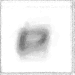
\includegraphics{building-mean}
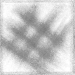
\includegraphics{dirt-mean}
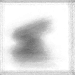
\includegraphics{forest-mean}
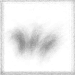
\includegraphics{grass-mean}
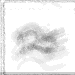
\includegraphics{water-mean}
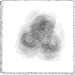
\includegraphics{rocks-mean}
\caption{The gold images created as the mean image of all examples of each symbol.
In order we have symbols representing buildings, dirt, forest, grass, water, and rocks.}
\label{figure:means}
\end{figure}

Similar to the feature-based approach, we define $x$ and $y$ to be the row and column sums
and calculate the mean and standard deviation of $x$ and $y$. To get the symbols to overlap we apply a
linear transformation to each pixel using the statistics gathered in each dimension.

\begin{equation} \label{eq:gold}
x^{\prime} = (x - \mu^{B}_{x}) \, \frac{\sigma^{G}_{x}}{\sigma^{C}_{x}} + \mu^{G}_{x} \quad
y^{\prime} = (y - \mu^{B}_{y}) \, \frac{\sigma^{G}_{y}}{\sigma^{C}_{y}} + \mu^{G}_{y}
\end{equation}

These new transformed pixels are placed into a new image $A$ which now overlaps with the
gold image $G$. We then compare the overlapping image $A$ to the gold standard image $G$ by taking the sum
of the squared difference at each pixel position. This gives us an error measure which we
record for each of the $k$ classes.

\[ \xi_{k}(A) = \sum_{i}\sum_{j}{(A_{ij} - G_{kij})^{2}} \]

The result is a vector of size $k$, the number of classes, with an error measure for the
comparison against the corresponding class. We then input this vector into WEKA along
with the correct answer for training purposes. We use a J48 decision tree with 10-fold
validation to train WEKA to classify using these error measures.

To create the gold images, we collected all the samples in our data set and 
created a mean gold image by overlapping all the smaples belonging to the same class,
the results can be seen in Figure \ref{figure:means}
